% Header: Here are all packages used and some additional definitions
%%%%%%%%%%%%%%%%%%%%%%%%%%%%%%%%%%%%%%%%%%%%%%%%%%%%%%%%%%%%%%%%%%%

\documentclass[11pt,a4paper]{article}
\usepackage[margin=2.5cm]{geometry}
\usepackage[onehalfspacing]{setspace}
\usepackage{graphicx} % zum Einbinden von Graphiken
\usepackage[breaklinks=true,colorlinks=true,linkcolor=blue,urlcolor=blue,citecolor=blue]{hyperref} % f. Referenzen
\usepackage{amsmath,amsthm,amssymb} % Mathematik Umgebung 
\DeclareMathOperator*{\argmax}{arg\,max}
\DeclareMathOperator*{\argmin}{arg\,min}


\usepackage{icomma} % Intelligentes Komma, das den richtigen Abstand zwischen Dezimalzahlen als auch in Formeln wählt.
%\usepackage[ngerman]{babel} % Deutsche Bezeichnungen bei Inhaltsangabe etc
\usepackage[T1]{fontenc}    % andere Schriftsatzkodierung für richtige Silbentrennung bei Umlauten
\usepackage[locale = DE,space-before-unit=true,per-mode = symbol]{siunitx} % Bessere Einheiten
\usepackage{placeins} % Definiert den Befehl “\FloatBarrier”, der die Ausgabe der davor eingebundenen Bilder erzwingt, befor der Text weiter geht. (Mit vorsicht zu verwenden)
%\usepackage[natbib,abbreviate=true,doi=false,style=numeric-comp,giveninits=true,sorting=none]{biblatex} % Modernes Paket zur Erzeugung von Bibliografien (benötigt biber!)
\usepackage[normalem]{ulem}
%\addbibresource{MyBibliography.bib} % Ort der .bib Datei, die die Datenbank für Literatur/Referenzen enthält.
\usepackage[ruled,vlined]{algorithm2e}
\SetKwInput{KwInput}{Input} % Set the Input
\SetKwInput{KwOutput}{Output} % set the Output
\graphicspath{{Bilder/}}

%\DeclareSIUnit{\dBm}{dBm}
%\DeclareSIUnit[per-mode=reciprocal]\WN{\per\centi\meter}


%Bibliography and citations
\usepackage[backend=biber, style=authoryear, sorting=nyt, maxnames = 10, maxcitenames = 2]{biblatex}
\addbibresource{references.bib}


\DeclareFieldFormat{citehyperref}{%
  \DeclareFieldAlias{bibhyperref}{noformat}%
  \bibhyperref{#1}}
\savebibmacro{cite}
\renewbibmacro*{cite}{%
  \printtext[citehyperref]{%
    \restorebibmacro{cite}%
    \usebibmacro{cite}}}

\let\cite\parencite

\AtBeginBibliography{\renewbibmacro*{begentry}{\printnames{author}}}
\AtEveryBibitem{\clearfield{note}}

\setlength{\bibhang}{1em}
%\defbibenvironment{bibliography}
%  {\list
%     {\printtext[labelnumberwidth]{%
%        \printfield{labelprefix}%
%        \printfield{labelnumber}}}
%     {\setlength{\labelwidth}{\labelnumberwidth}%
%     \setlength{\leftmargin}{\bibhang}
%     % \setlength{\leftmargin}{\labelwidth}%
%      \setlength{\labelsep}{\biblabelsep}%
%      \setlength{\itemsep}{\bibitemsep}%
%      \setlength{\parsep}{\bibparsep}%
%      \addtolength{\leftmargin}{\labelsep}%
%      \setlength{\itemindent}{-\bibhang}
%      %\setlength{\itemindent}{0pt}%
%      \renewcommand*{\makelabel}[1]{\hss##1}%
%      \raggedright}}
%  {\endlist}
%  {\item}

 

%%%%%%%%%%%%%%%%%%%%%%%%%%%%%%%%%%%%%%%%%%%%%%%%%%%%%%%%%%%%%%%%%%%
\begin{document}
%
\title{Bayesian Hierarchical CRR}
\author{Sophie Huebler \thanks{\href{mailto:sophie.huebler@utah.edu}{sophie.huebler@utah.edu}}}
\date{\today}
\maketitle
%\vfill
\pagenumbering{arabic} 
\tableofcontents

\newpage
\section{Motivation}
\label{sec:Motivation}
The presence of competing risks in time to event outcome data necessitates a high dimensional survival model that can identify prognostic variables for an event of interest, even when the relationship between the hazard function and the cumulative incidence function is complicated by the competing risk. \\
\textit{Why this works:
\begin{itemize}
    \item Highlights why competing risks are a problem (complicates the relationship between the hazard function and CIF)
    \item States the main hypothesis of the model (it will be good at identifying prognostic variables)
    \item Motivates how we may investigate the performance of our model 
    \begin{itemize}
        \item Situation: when competing risks complicate the relationship between the hazard and CIF
        \item Assessment: can we still identify important variables (variable selection) and are they prognostic (prediction)
    \end{itemize}
\end{itemize}
}
\subsection{Statistical Gap}
Penalization methods that rely on adaptive shrinkage applied directly to regression coefficients tend to either overshrink all coefficients, as is the case with LASSO  \cite{FanLi2001}, or only perform unbiased estimation for large coefficients, as is the case with SCAD \cite{ZouLi2008}. Spike-and-slab LASSO models introduce a latent probability of inclusion parameter which allows for even small coefficients to be kept, even as the penalization parameter grows \cite{RockovaGeorge2018}, but spike-and-slab LASSO does not currently exist for a competing risks framework. 


%\thispagestyle{empty}
%
%

%\thispagestyle{empty}
%\cleardoublepage
\newpage
%

\section{Introduction}
\label{sec:Intro}

\subsection{Clinical motivation}
\textit{
This section should motivate the general goal of identifying prognostic features from omics data for therapeutic or knowledge discovery.
\begin{itemize}
    \item Omics data in a clinical setting gives us a large number of potential targets to investigate as therapeutic intervention points or as evidence of mechanistic relationships between biological pathways and disease processes \parencite[]{Sibilio2025, IvanisevicSewduth2023} 
    \begin{itemize}
        \item Eg. Finding a set of gut microbial features that increase the risk of GVHD could result in a targeted antibiotic regimen. 
        \item Eg. Finding a set of upregulated genes associated with relapse at x days after treatment could result in a better understanding of how a certain metabolic pathway relates to a certain disease 
    \end{itemize}
    \item It is expensive and time consuming to investigate all targets \cite{Dibyajyoti2013}, so we need a way to narrow down the number of targets to investigate, and we want to keep targets with small signals as well as large to maximize the possibility of finding a good target/set of targets (CITE?).
    \item Time to event outcomes are common. Especially if we are looking for intervention targets \cite{SchoberVetter2018}(?), a survival analysis setting directly provides baseline as the intervention time.
\end{itemize}
}
As genomic data becomes more available in clinical settings, high dimensional techniques capable of modeling patient outcomes must preserve interpretability in order to translate into targets for intervention. Additionally, a model must be capable of identifying small effects. 

\subsection{Regularization}
\textit{
This section should clarify and explain why we are working in the context of regularization.
\begin{itemize}
    \item Regularization is a form of variable selection in high dimensional settings \cite{Hastie2015} 
    \item Regularized regression is straightforward to interpret, and feature importance is inherant to the process rather than being post-hoc \cite{Hastie2015} 
    \item We prefer regularization over black box machine learning type models for inference (opinion?)
    \item Regularization is a likelihood based method
\end{itemize}
}

Regularization methods allow for variable selection, which is critical for drawing inference from a high dimensional predictive model \cite{Hastie2015} . They are capable of simultaneously performing variable selection and estimating conditional effects among a set of many features . 

\subsubsection{Regularization techniques}
\textit{
This section should discuss regularization methods (as defined by their penalty terms) and their benefits and drawbacks. It should end with SSL as a good method for variable selection with small signals and a lot of noise.
\begin{itemize}
    \item Regularization techniques are defined by their penalty terms \cite{Hastie2015} 
    \item Describe LASSO \cite{Tibshirani1997}
    \item Describe problem with LASSO overshrinking \cite{FanLi2001, Zou2006, Ghosh2016}
    \item Describe adaptive shrinkage LASSO \cite{Zou2006, ZhangLu2007}  and under what circumstances it improves overfitting
    \item Describe SCAD and maybe other convex penalty terms \cite{FanLi2001} 
    \item Describe problems with SCAD with small coefficients \cite{ZouLi2008} 
    \item Describe SSL \cite{RockovaGeorge2018, Bai2020} 
    \item Emphasize how SSL allows selection of small coefficients \cite{RockovaGeorge2018} 
\end{itemize}
}
Different penalization methods include [List here with citations: LASSO, SCAD, ect], with adaptive shrinkage methods performing well under sparsity conditions \cite{ZhangLu2007}. 
\subsubsection{Bayesian regularization}
\textit{This section should describe how a penalty term can be translated into a bayesian hierarchical framework using priors.
\begin{itemize}
    \item Penalty terms can be converted to bayesian priors \cite{ParkCasella2008}
    \item MAP estimate is equivalent to MLE \cite{IshwaranRao2005, Bai2020}
    \item LASSO is a double exponential prior \cite{ParkCasella2008, YiXu2008}
    \item SSL is a double exponential mixture prior \cite{RockovaGeorge2018}
    \item Methods exist for fitting Bayesian hierarchical models using EM cyclic coordinate descent \cite{RockovaGeorge2014, Simon2011}
\end{itemize}
}

\subsection{Survival}
\textit{
This section should briefly introduce the proportional hazards framework, emphasizing that true target is the CIF and how the hazard has a direct relationship.
\begin{itemize}
    \item Often times, the primary quantities of clinical interest in a survival analysis are conditional covariate effects on the marginal probability of a certain outcome event, measured by the cumulative incidence function (CIF). 
    \item The cox partial likelihood has direct parameter relationship between CIF and hazard (Cox1972) 
    \item Cox gives a partial likelihood for survival outcome data which can be penalized \cite{VerweijHouwelingen1994, FanLi2002} 
    \item In single risk setting, the relationship between the covariate effects on the hazard function, as estimated by the Cox model, are directly, monotonically related to the covariate effects on the CIF.
    \item SSL in cox \cite{Tang2017}
\end{itemize}
}
\subsubsection{Competing risks}
\textit{
This section should describe how competing risks complicates the relationship of effects on hazard with the effects on CIF.
\begin{itemize}
    \item Single risk settings are rare \cite{AustinFine2017}  and especially rare in vulnerable populations
    \item Direct relationship breaks down when effects are in the same direction, greater magnitude, for competing event over event of interest \cite{Andersen2012}
    \item PSDH reinstates the relationship \cite{FineGray1999} with the scale of the regression coefficients on the PHS actually indicates whether an increase in covariate is associated with increase/decrease in the incidence of the event, but does not measure effect size on the probability of the occurrence of an event \cite{Monterrubiogomez2023}
    \item PSDH can be penalized  \cite{Fu2017}
    \item PH cannot hold in cause specific and competing risk at the same time \cite{Grambauer2010}
\end{itemize}
}
Single-risk settings can be rare in clinical settings, especially in high risk populations where mortality can be a common competing risk . In such cases, the monotonic relationship between covariate effects on the hazard function and on the CIF break down \cite{FineGray1999} . The proportional subdistribution hazards model (PDSH), or Fine-Gray model, is the standard extension to the Cox model, establishing a semiparametric framework to draw valid inference on the CIF from the subdistribution hazard function \cite{FineGray1999}. 



\subsection{Proposal}
We propose a Bayesian SSL model built around the proportional subdistribution hazards model to efficiently estimate maximum a posteri conditional covariate effects of high dimensional predictors on time-to-event outcomes with competing risks. The following sections will [2] outline the model and the adapted EM coordinate descent algorithm to fit the model, [3] describe the planned simulation and real data applications of the model. 


\newpage
\section{Methods}
\subsection{PSH}
Here, we consider a right censored survival scenario with two possible failure events, adopting notation from \cite{FineGray1999}. We call the failure type $\epsilon \in \{1,2\}$ such that $\epsilon = 1$ designates the failure as the event of interest and $\epsilon = 2$ designates the failure as the competing event. We call $T$ and $C$ failure and censoring times respectively, where $T$ can be failure from either event. Let $\Delta = I(T \leq C)$ be a non-censoring indicator, where $I(\cdot)$ is the indicator function, such that $\Delta = 1$ only if no failure event is observed. Then for each individual $i$, we observe $\{X_i, \Delta_i, \Delta_i \epsilon_i, \mathbf{z_i}\}$, where $X_i = \min(T_i, C_i)$ and $\mathbf{z_i}$ is a $J \times 1$ vector of covariates.  \\

 The cummulative incidence function (CIF) of the event of interest, conditional on covariates $\mathbf{z}$, is $F_1(t;\mathbf{z}) = P(T \leq t, \epsilon = 1 | \mathbf{z})$. Understanding how covariates affect this quantity is the modeling goal. The framework developed by \cite{FineGray1999} constructs a subdistribution hazard function $h_1$ for an artificially defined population such that the proportional hazards specification of $h_1$ directly relates to the true CIF of the event of interest through the $J \times 1$ vector of regression coefficients $\boldsymbol{\beta}$ and a baseline hazards function $h_{10}$:
 \begin{align*}
     h_1(t ; \mathbf{z}) & = \lim_{\Delta t \rightarrow 0} \frac{1}{\Delta t} \Pr(t \leq T \leq t + \Delta t, \epsilon = 1 | T \geq t \cup (T \leq t \cap \epsilon \ne 1), \mathbf{z})\\
     & = \{dF_1(t;\mathbf{z})/dt\}/(1-F_1(t;\mathbf{z}))\\
     & = h_{10}(t) \exp (\mathbf{z}^T\boldsymbol{\beta})
 \end{align*}

The resulting partial psuedo-loglikehood for the  Proportional Subdistribution Hazard (PSH) model is defined in terms of a counting process, $N_i(t) = I(T_i \le t, \epsilon_i = 1)$, and an at risk of the event of interest process, $Y_i(t) = 1 - N_i(t-)$:

\begin{align*}
    l_p(\boldsymbol{\beta}) = \sum_{i=1}^n \int_0^{\infty} &\left[\mathbf{z_i}^T\boldsymbol{\beta}-\log \left\{ \sum_q w_q(u)Y_q(u) \exp (\mathbf{z_q}^T\boldsymbol{\beta}) \right\}  \right] \\ &\times w_i(u)dN_i(u)
\end{align*}
\noindent
where the time dependent weights, $w$, arise from inverse probability of censoring weights (IPCW) \cite{RobinsRotnitsky1992} based on the survival function of the censoring variable $G(t) = Pr(C \ge t)$. The Kaplan-Meier estimate $\hat{G}(t)$ is employed such that $w_i(t) = \frac{I(C_i \ge \min(T_i, t))\hat{G}(t)}{\hat{G}(\min(T_i, t))}$.\\


When extending the PSH model in high-dimensional setting, LASSO regularization can be applied by maximizing the partial pseudo-loglikelihood with an $L_1$ penalty term applied: \cite{Hastie2015, Simon2011, Tibshirani1997, Fu2017}.
\begin{align*}
    p\ell_p(\boldsymbol{\beta}) = \ell_p(\boldsymbol{\beta}) - \lambda\sum_{j=1}^J|\beta_j|
\end{align*}

The penalty parameter $\lambda$ controls the shrinkage of the parameters, with adaptive shrinkage methods utilizing parameter specific $\lambda_j$ values to control the amount of shrinkage \cite{Zou2006, ZhangLu2007}. Cyclic coordinate descent algorithms for the psh model estimate parameters by maximizing $p\ell_p(\boldsymbol{\beta})$ \cite{Fu2017}, and recent advances allow for the model to be fit in linear time using a forward backward scanning procedure \cite{Kawaguchi2021, Kawaguchi2020}. 

\subsection{Spike-and-slab LASSO Priors}
It can be useful to interpret LASSO penalized least squared regression problems in a Bayesian hierarchical framework. The $L_1$ penalized estimates can be approximated by posterior mode estimates for regression parameters with independent, identically distributed double-exponential priors on the coefficients \cite{ParkCasella2008, YiXu2008}:
\begin{align*}
    %\beta_j|s \sim \mathrm{DE}(\beta_j|0,s)
    p(\boldsymbol{\beta}|s)= \prod_{j=1}^J \frac{s}{2}\exp[-s|\beta_j|] 
\end{align*}
\noindent
where the scale parameter of the double-exponential distribution $s$ is equal to $\lambda^{-1}$, the inverse of the penalty parameter. 

We employ spike-and-slab LASSO priors \cite{RockovaGeorge2018}, which arise from extending the LASSO prior from a single double-exponential prior to a spike-and-slab mixture double exponential prior:
\begin{align*}
p(\boldsymbol{\beta}|\boldsymbol{\gamma})= \prod_{j=1}^J[(1-\gamma_j)\psi(\beta_j|s_0) + \gamma_j\psi(\beta_j|s_z)]
%\beta_j|\gamma_j,s_0,s_1 \sim (1-\gamma_j)\mathrm{DE}(\beta_j|0,s_0)+\gamma_j\mathrm{DE}(\beta_j|0,s_1)
\end{align*}

\noindent
where $\psi(\beta|s) = 1/(2s)e^{-|\beta_j|/s}$ is the density function for the double-exponential distribution with a scale parameter $s$, and $\gamma_j$ is a binary indicator variable for coefficient $j$ belonging to either the spike distribution, characterized by scale $s_0$, or the slab distribution, characterized by scale $s_1$. This formulation is so called because it bridges the spike-and-slab paradigm and the LASSO paradigm. When the scales of the mixture distributions are chosen such that $s_0=s_1$, the priors reduce to the original LASSO priors. However, when the scales are chosen such that $s_0 < s_1$, the priors mix to LASSO terms adaptively such that strong shrinkage is applied to irrelevant coefficients, sampling them from the spike distribution which pulls the estimates towards $0$, and weak shrinkage is applied to influential coefficients by pulling them into the slab distribution.

We assume that the coefficient specific indicator variables, $\gamma_j$, is sampled from Bernoulli distribution condictioning on a probability parameter $\theta$, the mixing proportion which controls the overall sparsity. Under the fully Bayesian hierarchical model, $\theta$ is designated as a random variable which allows for the model to self-adapt to sparsity in the data \cite{RockovaGeorge2018, Castillo2012} \textit{(Add proofs into a \textcolor{blue}{supplement}? Maybe describing marginal dependence among the betas and how this turns into a non-separable penalty)}. We place a beta prior on $\theta$ to exploit the beta-binomial conjugacy. The full specification of the Bayesian hierarchical spike-and-slab LASSO priors is as follows:

\begin{align*}
    \beta_j \mid \gamma_j, s_0, s_1 &\sim (1 - \gamma_j)\text{DE}(\beta_j \mid 0, s_0) + \gamma_j\text{DE}(\beta_j \mid 0, s_1) \\
    \gamma_j| \theta &\sim \text{Bernoulli}(\theta) \\
    \theta &\sim \text{Beta}(a,b)
\end{align*}




\subsubsection{Properties of spike-and-slab LASSO}
\begin{itemize}
    \item We note here, as is demonstrated in \cite{RockovaGeorge2018}, that the spike-and-slab LASSO induces adaptive regularization such that different shrinkage is applied to individual coefficients. 

    \item The conditional probability that $|\beta_j|$ was drawn from the slab distribution rather than the spike distribution, conditional on the estimated overall sparsity $\hat\theta$, is an exponentially increasing function of the $|\beta_j|$:
\begin{align*}
    \Pr(\gamma_j = 1|\beta_j, \hat{\theta}) = \frac{1}{1+\frac{(1-\hat \theta)s_0}{\hat \theta s_1}\exp(-|\beta_j|(s_0-s_1))}
\end{align*}

\item We can set parameter specific mixture $S_j = (1-\gamma_j)s_0 + \gamma_js_1$. Then the prior expectation $E(S_j) = (1-\theta)s_0 + \theta s_1 \in [s_0,s_1]$. We note that \begin{align*}
    \beta_j | \gamma_j, s_0, s_1 &\sim (1 - \gamma_j)\text{DE}(\beta_j \mid 0, s_0) + \gamma_j\text{DE}(\beta_j \mid 0, s_1) 
    \\ & \sim \mathrm{DE(\beta_j|0, S_j)}
\end{align*}

\item We let $a=b=1$ such that $\theta \sim \mathrm{Beta}(1,1) = \mathrm{Unif(0,1})$. This is a naive prior, such that we are not suggesting a prior level of sparsity. This term constants out of the log joint posterior density. But we still use the beta-binomial conjugacy for the form of the gamma prior. \cite{Castillo2012, RockovaGeorge2018} suggest setting $a=1, b=p$ as a common level to induce a high degree of sparsity.

\end{itemize}





\subsection{Algorithm}
Techniques for Bayesian variable selection through expectation-maximization were developed in \cite{RockovaGeorge2014} to deterministically identify sparse high posterior probability submodels from high dimensional data by using conjugate mixture prior formulations to calculate posterior modes. An adaptation of the algorithm tailored to survival data was further developed in \cite{Tang2017} to handle single-cause time-to-event data under a Cox proportional hazards framework using expectation-maximization with cyclic coordinate descent. We utilize the algorithm once more, this time incorporating competing risks. Our contributions to the methodology are specifically incorporating competing risks through the substitution of the Cox likelihood with the PSH likelihood, making it necessary to use a different the cyclic coordinate descent algorithm, as well as through the use of competing risk aware evaluation metrics for tuning purposes. 
\subsubsection{Joint posterior density}
The EMCCD is based on the log joint posterior density of the parameters $(\boldsymbol{\beta}, \boldsymbol{\gamma}, \theta)$. We first recognize the proportionality of the joint posterior density with the product of the data likelihood and the prior density functions:
\begin{align*}
    p(\boldsymbol{\beta}, \boldsymbol{\gamma}, \theta| \{X_i, \Delta_i, \Delta_{i}\epsilon_i, \mathbf{z_i}\}) \propto p(\{X_i, \Delta_i, \Delta_{i}\epsilon_i, \mathbf{z_i}\}| \boldsymbol{\beta}, h_{10})\times p(\boldsymbol{\beta}|s_0, s_1, \boldsymbol{\gamma}) \times p(\boldsymbol{\gamma}|\theta) \times p(\theta)
\end{align*}
\noindent Then, finding the log joint posterior density, we make the substitution that $\log p(\{X_i, \Delta_i, \Delta_{i}\epsilon_i, \mathbf{z_i}\}|\boldsymbol{\beta}, \boldsymbol{\gamma}, \theta) \propto \ell_p(\boldsymbol{\beta})$ and $S_j = (1-\gamma_j)s_0 + \gamma_js_1$ to get the following:
\begin{align*}
    & \log p(\boldsymbol{\beta}, \boldsymbol{\gamma}, \theta| \{X_i, \Delta_i, \Delta_{i}\epsilon_i, \mathbf{z_i}\})
     \\ & \propto \ell_p(\boldsymbol{\beta}) + \sum_{j=1}^J \log p(\beta_j|S_j)+ \sum_{j=1}^J  \log p(\gamma_j|\theta) + \log p(\theta)
     \\ & \propto \ell_p(\boldsymbol{\beta})
    - \sum_{j=1}^{J} \frac{1}{S_j} \lvert \beta_j \rvert + 
    \sum_{j=1}^{J}\left(\gamma_j \log \theta + (1 - \gamma_j)\log(1 - \theta)\right)
\end{align*}

\noindent where $p(\theta) \sim \mathrm{Beta(1,1)} = \mathrm{Unif}(0,1)$.  (\textit{Add further derivations into a \textcolor{blue}{supplement}? If so maybe work out the generalized distribution with a beta prior on theta. Also need to convince myself it is ok to proportion out the 1/(2s) term from the ssl priors. })


\subsubsection{EM algorithm}
\textit{write 1. The justification/intuition of using EM algorithm; 2. one sentence descirption of what is EM algorithm}

We treat the indicator variables $\boldsymbol{\gamma}$ to be missing variables. We will use the cyclic coordinate descent expectation maximization framework from \cite{Tang2017}, wherein we iteratively maximize the expectation of a separable objective  with respect to the posterior distribution of our latent variables. We adopt the notation of \cite{RockovaGeorge2014} to define the objective function in terms of log joint posterior density of the parameters  conditional on the posterior distribution of our latent variables:
\begin{align*}
    &Q(\boldsymbol{\beta}, \theta|\boldsymbol{\beta}^{(k)}, \theta^{(k)}) = E_{\boldsymbol{\gamma}|\cdot}\left[ \log p(\boldsymbol{\beta}, \boldsymbol{\gamma}, \theta| \{X_i, \Delta_i, \Delta_{i}\epsilon_i, \mathbf{z_i}\})| \boldsymbol{\beta}^{(k)}, \theta^{(k)},\{X_i, \Delta_i, \Delta_{i}\epsilon_i, \mathbf{z_i}\} \right]
\end{align*}
\noindent where $E_{\boldsymbol{\gamma}|\cdot^{(k)}}(\cdot) = E_{\boldsymbol{\gamma}|\boldsymbol{\beta}^{(k)}, \theta^{(k)},\{X_i, \Delta_i, \Delta_{i}\epsilon_i, \mathbf{z_i}\}}(\cdot)$

We note that the form of the objective function is decomposable, with one portion corresponding to a regularized PSH model and one portion corresponding to the beta-binomial conjugate prior \textit{rephrase} on the latent indicator variables:
\begin{align*}
    Q(\boldsymbol{\beta}, \theta|\boldsymbol{\beta}^{(k)}, \theta^{(k)}) = Q_1(\boldsymbol{\beta}|\boldsymbol{\beta}^{(k)}, \theta^{(k)})  + Q_2( \theta|\boldsymbol{\beta}^{(k)}, \theta^{(k)})
\end{align*}

where 
\begin{align*}
    Q_1(\boldsymbol{\beta}|\boldsymbol{\beta}^{(k)}, \theta^{(k)}) = \ell_p(\boldsymbol{\beta})
    - \sum_{j=1}^{J} E_{\boldsymbol{\gamma}|\cdot^{(k)}}(S_j^{-1}) \lvert \beta_j \rvert
\end{align*}

and

\begin{align*}
    Q_2( \theta|\boldsymbol{\beta}^{(k)}, \theta^{(k)}) = \sum_{j=1}^{J}\left[E_{\boldsymbol{\gamma}|\cdot^{(k)}}(\gamma_j) \log \theta + (1 - E_{\boldsymbol{\gamma}|\cdot^{(k)}}(\gamma_j))\log(1 - \theta)\right]
\end{align*}


For the E step, we calculate the conditional expected value of the latent variables, and then the conditional expected value of the penalty weights which depend on the latent variables. We condition on the current parameter values, noting that for any given iteration $(k)$, the conditioning set $\boldsymbol{\beta}^{(k)}, \theta^{(k)}$ is made up of fixed values and the latent variables depend on the data only through those values. We take the expectation with respect to the posterior distribution of the latent variables. For each individual parameter, we find $p^{(k)}_j = E_{\boldsymbol{\gamma}|(\boldsymbol{\beta}^{(k)}, \theta^{(k)})}$, which is equal to the probability that $B_j$ comes from the slab component of the mixture distribution: 
\begin{align*}
     p^{(k)}_j = &E_{\boldsymbol{\gamma}|(\boldsymbol{\beta}^{(k)}, \theta^{(k)})}\gamma_j\\
     =& \Pr(\gamma_j = 1 | \boldsymbol{\beta}^{(k)}, \theta^{(k)})
     \\=  &  \frac{\pi(\beta_j^{(k)} \mid \theta^{(k)}, \gamma_j = 1) \cdot \pi(\theta^{(k)} \mid \gamma_j = 1) \cdot \Pr(\gamma_j = 1)}{\int_{\gamma_j} \pi(\beta_j^{(k)}, \theta^{(k)})d\gamma_j}
     \\=& \frac{a_j^{(k)}}{a_j^{(k)} + b_j^{(k)}}
\end{align*}

\noindent where $a_j^{(k)} = \pi(\beta_j^{(k)}| \gamma_j = 1)\Pr(\gamma_j = 1 | \theta^{(k)})$ is the joint density that the current $\beta_j^{(k)}$ comes from the slab distribution, and $b_j^{(k)} = \pi(\beta_j^{(k)}|\gamma_j = 0)\Pr(\gamma_j = 0 | \theta^{(k)})$ is the joint density that the current $\beta_j^{(k)}$ comes from the spike distribution. Dividing $a_j^{(k)} /(a_j^{(k)} + b_j^{(k)})$ gives the probability that $\beta_j$ comes from the slab distribution, so we call $p^{(k)}_j$ the posterior inclusion probability. Then using the posterior inclusion probability we can find the expected value of the penalty weights, which we will call $\lambda_j^{(k)}$:
\begin{align*}
    \lambda_j^{(k)} &= E_{\boldsymbol{\gamma}|(\boldsymbol{\beta}^{(k)}, \theta^{(k)})}(S^{-1 }_j|\beta_j^{(k)}) 
    \\& = \sum_{x \in \{0,1 \} }\left[\frac{1}{(1-x)s_0 + xs_1} E_{\boldsymbol{\gamma}|(\boldsymbol{\beta}^{(k)}, \theta^{(k)})}(\gamma_j = x)\right]
    \\ & = \frac{1-p^{(k)}_j}{s_0} + \frac{p^{(k)}_j}{s_1}
\end{align*}

For the M step, we separately maximize the components of the objective function. Maximizing $Q_2$ updates the mixing proportion $\theta$. The solution is closed form, with the updated mixing proportion equal to the average of the posterior inclusion probabilities:
\begin{align*}
    \theta^{(k+1)}= \argmax_{\theta} \frac{1}{J}\sum p_j^{(k)}
\end{align*}

\noindent On the other hand, $Q_1$ does not have a closed form solution, but it takes the form of LASSO penalized PSH model where the penalty weights are $\lambda^{(k)}$:

\begin{align*}
    \boldsymbol{\beta}^{(k+1)}= \argmax_{\boldsymbol{\beta}} \ell_p(\boldsymbol{\beta}) - \lambda^{(k)}\sum_{j=1}^J |\beta_j|
\end{align*}
This can be estimated using cyclic coordinate descent algorithm. Specifically, \cite{Kawaguchi2020} provides an extremely fast cyclic coordinate descent algorithm for the PSH model by using a forward-backward scanning algorithm that exploits the monotonicity of time-dependent disjoint risk sets. This algorithm is implemented in the fastcmprsk package in R \cite{Kawaguchi2021}, and it allows for independently supplied penalty weights.

In full, the EM algorithm proceeds as follows:

\begin{algorithm}[h]
\label{EM}
\DontPrintSemicolon
 
\KwInput{Data $\{\boldsymbol{X}_{n \times 1}, \boldsymbol{\Delta}_{n \times 1}, [\boldsymbol{\Delta}\boldsymbol{\epsilon}^T]_{n \times 1}, \mathbf{Z}_{n \times J}\}$; Hyperparameters $s_0$ and $s_1$; Initial estimates $\boldsymbol{\beta_0}, \theta_0$; Convergence threshold $\epsilon$ }
\KwOutput{Estimated regression coefficients}\;
\BlankLine
\textbf{Initialize:} $t \leftarrow 0$, $\boldsymbol{\beta}^{(0)} \leftarrow \boldsymbol{\beta_0}$, $\boldsymbol{\theta}^{(0)} \leftarrow \theta_0$\;
\BlankLine


\Repeat{$\frac{|d^{(t)} - d^{(t-1)}|}{0.1 - |d^{(t)}|} < \epsilon$}{
   
    
    \textbf{E-step}\;
    \begin{enumerate}
        \item Update each $p_j^{(t)}$ by conditional posterior expectation of $\gamma_j$
        \item Update each $\lambda_j^{(t)}$ by conditional posterior expectation of $S^{-1}_j$
    \end{enumerate}

     $t \leftarrow t + 1$\;
    
    \textbf{M-step}\;
    \begin{enumerate}
        \item Update $\theta^{(t)}$\;
        \item Update $\boldsymbol{\beta}^{(t)}$ using the cyclic coordinate descent algorithm\;
    \end{enumerate}
    
    Calculate the estimate of deviance: $d^{(t)} = \ell_p(\beta^{(t)})$\;
}


\Return{$\boldsymbol{\hat{\beta}} = \boldsymbol{\beta}^{(t)}$}
\caption{EM algorithm with cyclic coordinate descent}
\end{algorithm}

\subsubsection{Initialization values}
\begin{itemize}
    \item \cite{Ng2011}
\end{itemize}



\subsubsection{Convergence}
\begin{itemize}
    \item Within each iteration, convergence of the cyclic coordinate descent algorithm used to fit the model is assessed primarily by parameter stability. Secondarily deviance check added as a stop gap for overfitting such that a 99\% increase in deviance breaks the cycle.
    \item Stopping criterion of the entire EM algorithm is taken from \cite{Tang2017}, defined by a minimum decrease in deviance across iterations. \textit{\textcolor{red}{This stopping criteria seems incorrectly implemented. }Recheck what is in the package. Why 'stabilize' by adding constant to denominator which may still cause division by 0 error?}
\end{itemize}

\subsubsection{Hyperparameter tuning}
Implementing this model requires pre-specified scales for the spike and slab distributions. Because a double-exponential prior induces a LASSO penalty where smaller scale values increase coefficient shrinkage \cite{Tibshirani1997}, the overall shrinkage intensity of the mixture prior depends heavily on the careful selection of both scales. When $s_0 = s_1$, the model reduces to the standard LASSO \cite{RockovaGeorge2018}; consequently, we impose the non-inclusive constraint $s_0 < s_1$. While the model can be refitted across a grid search of parameters subject to this order constraint, selecting specific values remains non-trivial. Recent studies found that varying the slab distribution scale yields negligible performance improvements \cite{Tang2017, Tang2019, Bai2020}, and therefore recommend to fix the slab scale and vary only the spike scale. The scale, or scales, are then selected based on optimization of predictive performance of the model according to defined criteria.

Besides a choice of predictive performance metric to optimize, this hyperparameter tuning also requires a paradigm for creating an internal validation set. We advise against split sample validation due to concerns of overfitting \cite{Collins2024, Steyerberg2018}, and instead advocate for a resampling approach. Specifically, we recommend the pre-validation approach \cite{TibshiraniEfron2002, Hastie2015}, which has been used for tuning in other spike-and-slab LASSO models \cite{Tang2017, Tang2019, Yi2019, GuoYi2022}. Pre-validation computes a cross-validated prognostic index for each individual using the following procedure:

\begin{algorithm}[H]
\DontPrintSemicolon
\SetAlgoLined
\KwData{Data $\{\boldsymbol{X}_{n \times 1}, \boldsymbol{\Delta}_{n \times 1}, [\boldsymbol{\Delta}\boldsymbol{\epsilon}^T]_{n \times 1}, \mathbf{Z}_{n \times J}\}$, Number of folds $K$}
\KwResult{Cross-validated prognostic indices $\hat{\boldsymbol{\eta}}_{n \times 1}$}

\BlankLine
Randomly split the data into $K$ subsets $\{D_1, D_2, \dots, D_K\}$ of roughly equal size\;

\For{$k \leftarrow 1$ \KwTo $K$}{
    Let $D_{(-k)}$ be the data excluding the $k$-th subset\;
    Fit the model using $D_{(-k)}$ to obtain coefficient estimates $\hat{\beta}^{(-k)}$\;
    
    \textbf{Calculate indices for individuals in the held-out fold}\;
    \For{each individual $i$ in subset $D_k$}
    {$\hat{\eta}_i = X_i \hat{\beta}^{(-k)}$ }\;
}
\Return{$\hat{\boldsymbol{\eta}}_{n \times 1}$}
\caption{Pre-validation Procedure}
\end{algorithm}

\noindent In this way, no individual's observed response is used in the creation of their cross-validated prognostic score. This dataset can then be used as an independent dataset for valid assessments of predictive performance \cite{TibshiraniEfron2002}.

\textit{is this hyperparameter tuning completed?}


\subsubsection{Evaluation of predictive performance}

Already implemented:
\begin{itemize}
    \item Concordance index for competing risks \cite{Wolbers2014}.

     For survival data, a c-index is an aggregate measure of discrimination based on pairs of individuals whose outcomes can be compared in a meaningful way \cite{Harrell1982}. In the case of a single risk setting, an evaluable pair is any two individuals where the individual who experienced the event first can be determined, ie. two individuals who experienced the event or one individual who experienced the event and one individual who was censored afterwards. However, in a competing risk setting, it is necessary to redefine the idea of concordance as it relates to individuals who may experience events other than the event of interest. For our model, we are interested in modeling a single event of interest. \cite{Wolbers2014} introduces an unbiased estimator for the time-dependent concordance measure for this situation which is only dependent on the CIF for the event of interest, and which defines concordance to be the probability at time $t$ that the estimated risk of person $i$ is higher than the estimated risk of person $j$, given that person $i$ has experienced the event of interest, and person $j$ has either experienced the competing event or is event free. Formally, this measure is defined as:
     \begin{align*}
         C_1(t) = P(M(t,X_i) > M(t,X_j) \mid \epsilon_i = 1 \text{ and } T_i \leq t\text{ and } (T_i < T_j \text{ or } \epsilon_j = 2))
     \end{align*}
     \noindent where $M(t,\cdot)$ is the prognostic score from the model being evaluated. This definition can be extended to include tied data \cite{YanGreene2008}. 
     
     Estimators of concordance in censored survival data that do not account for the data left out from non-evaluable pairs are biased \cite{Uno2011, Gerds2012}. The estimator presented in \cite{Wolbers2014} employs inverse probability of censoring weighting to incorporate information from non-evaluable pairs by way of the censoring survival function, thereby eliminating the bias. Below is the procedure to estimate this quantity:
     <See algorithm \ref{algo:ipcw_cindex}>

     Any singular time point at which the c-index is taken is considered the truncation point. We select the median of the marginal distribution of event times as our truncation point, making this choice from among the options presented in \cite{Wolbers2014}. We note that the marginal distribution of event times is comprised of times corresponding to both the event of interest as well as the competing event, but not the censoring times. \textit{\textcolor{red}{Need to change in code to only evaluate event times}}.

     
     \end{itemize}

    

     
     \begin{algorithm}
\DontPrintSemicolon
\SetAlgoLined
\KwData{Observation times $\tilde{T}$, Status indicators $\tilde{\epsilon}$ (1=Event, 2=Competing, 0=Censored), Prognostic scores $M$, Evaluation time $t$, Sample size $n$}
\KwResult{Truncated concordance index $\hat{\mathcal{C}}_1(t)$}
\BlankLine
\textbf{Step 1: Estimate Censoring Distribution}\;
Define censoring indicator $\Lambda^C_i = I(\tilde{D}_i = 0)$ for all $i = 1, \dots, n$\;
Compute Kaplan-Meier estimate $\hat{G}(\tau)$ for censoring distribution using $(\tilde{T}, \Lambda^C)$\;
\BlankLine
\textbf{Step 2: Initialize Numerator and Denominator}
$Num \gets 0$\;
$Den \gets 0$\;
\BlankLine
\textbf{Step 3: Iterate over all pairs $(i, j)$}\;
\For{$i \gets 1$ \KwTo $n$}{
    \textbf{Check if subject $i$ is an evaluable case at time $t$}\;
    $\tilde{N}_i^1(t) \gets I(\tilde{T}_i \leq t \text{ and } \tilde{D}_i = 1)$\;
    \If{$\tilde{N}_i^1(t) == 0$}{
        \Continue\;
    }
    \For{$j \gets 1$ and $j \ne i$ \KwTo $n$}{
        %\If{$i == j$}{
        %    \Continue\;
        %}
        \textbf{Determine if pair is evaluable}\;
        $\tilde{A}_{ij} \gets I(\tilde{T}_i < \tilde{T}_j)$\;
        $\tilde{B}_{ij} \gets I(\tilde{T}_i \geq \tilde{T}_j \text{ and } \tilde{D}_j = 2)$\;
        Require $\tilde{A}_{ij}$ or $\tilde{B}_{ij}$
        %\If{$\tilde{A}_{ij} == 0$ \textbf{and} $\tilde{B}_{ij} == 0$}{
        %    \Continue\;
        %}
        
        \textbf{Calculate IPCW Weights}\;
        $W_{ij} \gets 0$\;
        \If{$\tilde{A}_{ij} == 1$}{
            $W_{ij} \gets [\hat{G}(\tilde{T}_i-) \times \hat{G}(\tilde{T}_i)]^{-1}$\;
        }
        \ElseIf{$\tilde{B}_{ij} == 1$}{
            $W_{ij} \gets [\hat{G}(\tilde{T}_i-) \times \hat{G}(\tilde{T}_j-)]^{-1}$\;
        }
        
        \textbf{Assess Concordance}\;
        $\mathcal{Q}^{ij}(t) \gets 0$\;
        \If{$M_i > M_j$}{
            $\mathcal{Q}^{ij}(t) \gets 1$\;
        }
        \ElseIf{$M_i == M_j$}{
            $\mathcal{Q}^{ij}(t) \gets 0.5$ \textbf*{Handling for tied risk scores}
        }
        
        \textbf{Accumulate weighted values}\;
        $Num \gets Num + (W_{ij} \times \mathcal{Q}^{ij}(t))$\;
        $Den \gets Den + W_{ij}$\;
    }
}
\KwResult{$\hat{\mathcal{C}}_1(t) = Num / Den$}
\caption{Calculation of the IPCW Cindex}
\label{algo:ipcw_cindex}
\end{algorithm}



To be implemented later:
\begin{itemize}
    \item Cross-validated partial log-likelihood \cite{Simon2011, Houwelingen2006} \textit{(Submitted ILL requests for (HouwelingenCessie1990, VerweijHouwelingen1993). Check if these support claim that CVPL is unbiased for Kullback-Leibler distance (Gemini-Thinking) as justification for using it as metric for how well model generalizes to new data from the underlying population.)} \\

    The cross-validated partial log likelihood (CVPL) is used to evaluate the generalizability of the predictive performance of a model by calculating the log-partial psuedo likelihood on held-out data across multiple cross-validation folds. The CVPL is calculated according to the following formula:
    \begin{align*}
        \mathrm{CVPL} = \sum^{K}_{k=1}\left[\ell_p(\hat{\boldsymbol{\beta}}_{-k}) - \ell_{p(-k)}(\hat{\boldsymbol{\beta}}_{-k})  \right]
    \end{align*}
    where $(\hat{\boldsymbol{\beta}}_{-k})$ is the vector of regression coefficients estimated by the model fit to data in all except the $k$th subset, $\ell_p(\hat{\boldsymbol{\beta}}_{-k})$ is the likelihood of the full data, and $\ell_{p(-k)}(\hat{\boldsymbol{\beta}}_{-k})$ is the likelihood of the data without the holdout subset. 

    \item Integrated brier score. 

    

    
\end{itemize}



\newpage
\section{Simulation}

\subsection{Overall goal}
The SSL PSH model will be more accurate than other regularization models in selecting for, and estimating the effect of, prognostic variables on survival outcome in the presence of competing risks.

\subsection{Comparison models}



\begin{table}[h]
    \centering
    \begin{tabular}{| c || c | c | c | c |}
    \hline
         & Correct Submodel & LASSO & SCAD & SSL \\
         \hline \hline
        Cox & survival::coxph & glmnet::glmnet & ncvreg::ncvsurv & BhGLM::bmlasso \\
        \hline
        PSH & cmprsk::crr & fastcmprsk::fastcrrp & fastcmprsk::fastcrrp & novel \\
        \hline
    \end{tabular}
    \caption{Model Comparisons: The package and function call of the different models we'll be testing}
    \label{tab:mods}
\end{table}

\subsubsection{Specific hypotheses we could check}
Function is coded to vary all of these scenarios quickly to test these hypotheses. 
\begin{itemize}
    \item As signal weakens, the SSL models will perform best in variable selection \\
    Reasoning:
    \begin{itemize}
        \item LASSO shrinks \cite{FanLi2001} 
        \item SCAD shrinks small coefficients  \cite{ZouLi2008}
        \item SSL does not shrink small coefficients \cite{Tang2017}
    \end{itemize}
    \item The PSH models will perform better than their cox counterparts in selecting for variables which affect both the event of interest and the competing event
    \begin{itemize}
        \item This difference in performance will be more apparent when the variables affecting both events affect the competing event in the same direction and with a greater magnitude\\
        Reasoning:
        \begin{itemize}
            \item \cite{Andersen2012}
        \end{itemize}
        \item This difference in performance will also be (different?) when the shape of the event of interest and the competing event differ\\
        Reasoning:
        \begin{itemize}
            \item This is just to check if we should vary the scenario
        \end{itemize}
        \item This difference in performance will be less apparent as censoring rate goes up\\
        Reasoning:
        \begin{itemize}
            \item Saw this in bamlasso \cite{GuoYi2022} (check if also in bmlasso?)
        \end{itemize}
    \end{itemize}
    \item As sparsity (the ratio of active predictors:inactive predictors) increases, the SCAD and SSL models will retain better predictive power than the LASSO models
    \item Hyperparameter tuning based on different metrics (cindex, MAE) will affect performance of SSL models\\
        Reasoning:
        \begin{itemize}
            \item This is just to check if we should vary the scenario
        \end{itemize}
\end{itemize}

\subsection{Assessment}
\subsubsection{Variable selection}
\begin{itemize}
    \item Sensitivity
    \begin{itemize}
        \item Find some precedent for weighted sensitivity where we care about sensitivity for a certain subset more? \cite{Hou2023}
    \end{itemize}
    \item Specificity 
\end{itemize}
\subsubsection{Predictive power}
\begin{itemize}
    \item Time dependent c-index at median survival time \cite{Wolbers2014}
    \item Cross-validated partial log-likelihood \cite{HouwelingenSauerbrei2013, Nicolaie2013, Houwelingen2006}
    \item Prevalidation \cite{TibshiraniEfron2002, Tang2017}
\end{itemize}


\subsection{Defining the outcome generating process}
\subsubsection{Inputs}
\begin{itemize}
    \item Number of competing events: 1
    \item Design matrix: Fixed 56 by 102 matrix. 
    \item Predictor set. Can either choose to supply 2 custom predictor sets (1 for the event of interest and 1 for the competing event) or can have have values chosen for you based on the following hyperparameters:
    \begin{itemize}
        \item Sparsity. A vector of length 2 that indicates how many predictors should actively affect event of interest and competing event respectively. 
        \item Shared predictors. A number indicating how many 'active' predictors should be shared between the event of interest and the competing event.
    \end{itemize}
    \item Regression coefficients. Can either choose to supply 2 custom resgression coefficient sets (1 for the event of interest and 1 for the competing event) or can have values chosen for you based on the following hyperparameters:
    \begin{itemize}
        \item The mean and standard deviation of the effects (corresponding to the distribution of the log odd ratios).
        \item  A target standard deviation of the linear predictors to control how heterogeneous the outcome is. 
        \item A vector of ratios < 1 (length = the number of shared predictors between the active sets for event of interest and competing event) such that for a shared predictor, the effect on the event of interest is ratio*effect on the competing event. 
    \end{itemize}
    \item The shapes and scales of the Weibull distributions for the event of interest and the competing event.
    \item The type of censoring (none, administrative at a certain day, or administrative at a certain day + randomly generated based on exponential distribution with a given rate parameter). 
\end{itemize}
\subsubsection{Choosing default inputs}
The default inputs were chosen to broach a range of scenarios. I chose to run a default scenario and let my function pick a set of active predictors and coefficients for me to use for each further defined scenario. Skip this section if uninteresting. 
\begin{itemize}
    \item Design matrix: Started with a design matrix from a real study (microbiome count table with psuedo count of 1 added and then centered log ratio transformed). Performed independent rowwise permutations such that columns (features) would not have a strong correlation structure. Columns were then mean centered. \\
    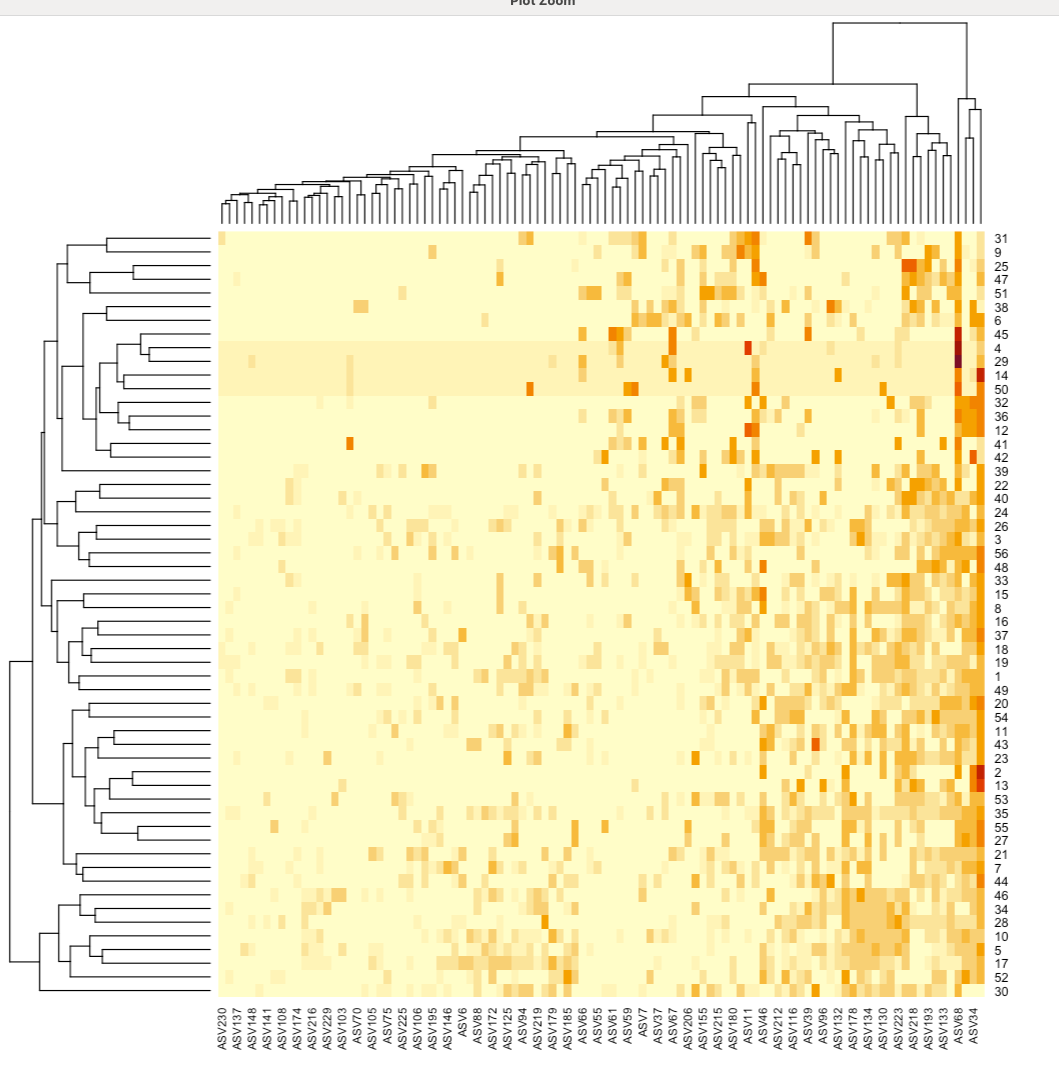
\includegraphics[width = 5cm]{Images/unpermuted_example_dat.png}
    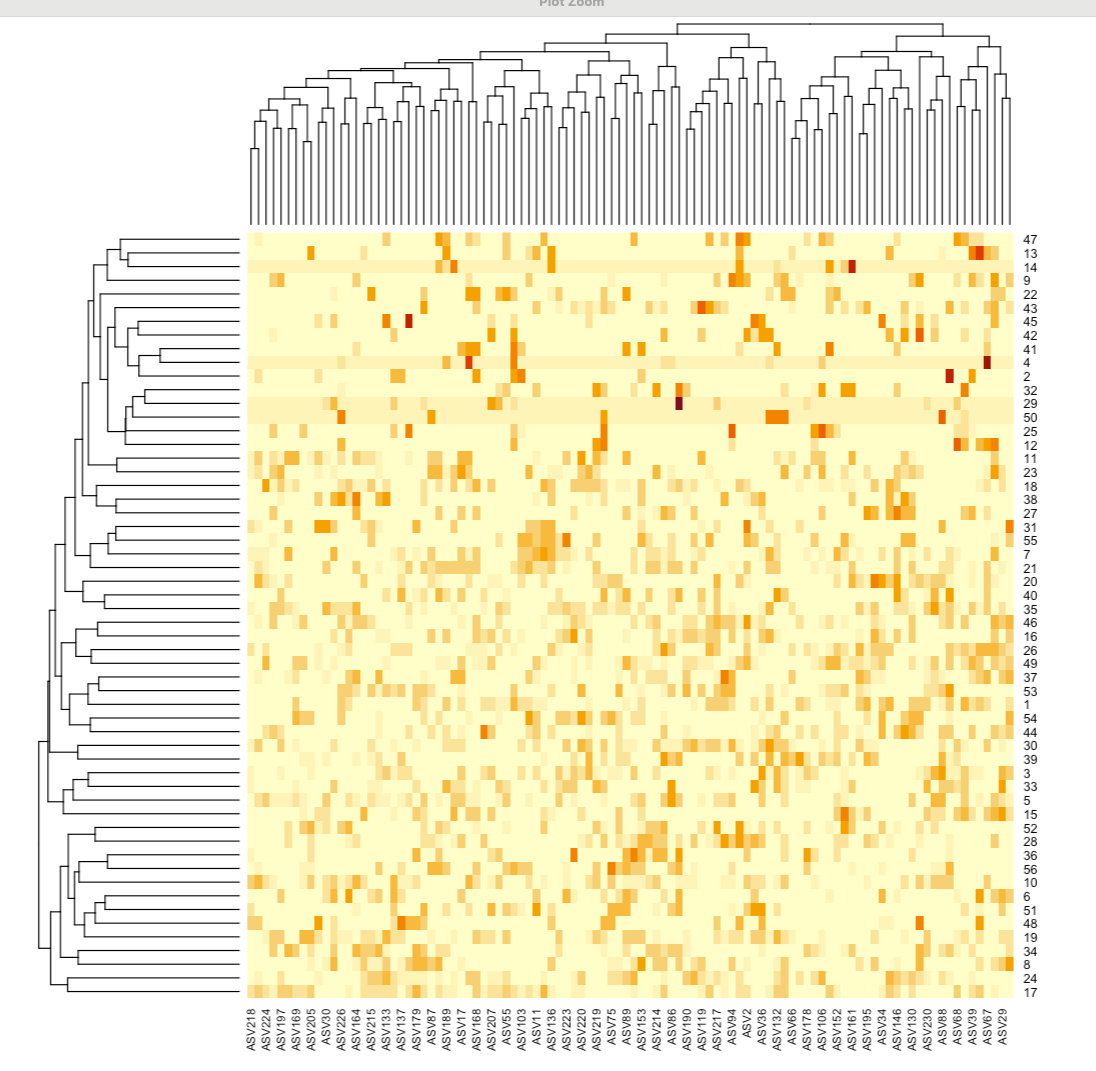
\includegraphics[width = 5cm]{Images/permuted_eample_dat.png}
    \item Predictor sets. Arbitrarily picked sparsity level of 0.05\% for event of interest and competing event such that each event had an active predictor set of size 6. Arbitrarily picked that the active predictor sets should overlap by 2. 
    \item Regression coefficients.
    \begin{itemize}
 
    \item Wanted to be able to control the latent survival times of the model. Under weibull propotional hazards model, survival time is given by 
    \begin{align*}
        S_i(t) = \exp(-\lambda t^{\gamma}\exp(\eta_i))
    \end{align*}
    where $\eta_i$ is the person specific linear predictor. Mean centering the columns of the design matrix means that $\bar{\eta}=0$, but with smallish sample size the heterogeneity in survival times was still large and the relative event rate (event of interest vs competing event) was inconsistent among runs. So used standard deviation of the linear predictors to constrain heterogeneity among outcome. This was done according to the following algorithm.
    \begin{itemize}
        \item Generate vector of $\beta^{[0]}_1$ from normal distribution with mean 0 and standard deviation of 0.3.
        \item Multiply by corresponding columns in design matrix to get a vector of linear predictors.
        \item Define scale factor = standard deviation of linear predictors/ target standard deviation
        \item Finalize $\beta^{[1]}_1 = \beta^{[0]}_1 \times$ scale factor
        \item If \# shared predictors = 0 then repeat as above for $\beta_2$
        \item Else calculate $\beta_2[shared] = \beta_1[shared]*1/ratio$
        \item Generate vector of $\beta^{[0]}_2[not shared]$ from normal distribution with mean 0 and standard deviation of 0.3.
        \item Calculate linear predictors as eta[shared] and eta[notshared]
        \item Solve for a scale factor for the not shared linear linear predictors by solving for c in \\ sd(eta[shared] + scale factor * eta[notshared]) - target standard deviation )**2 = 0
        \item Rescale the not shared betas by that scale factor
    \end{itemize}
    \item Wanted to ensure that the predictors in the overlap set had a stronger effect (in the same direction) on the competing event so chose a moderate difference in ratios (log odds ratio of first of the shared variables was half on the event of interest compared to the competing risk, log odds ratio of second of the shared variables was a fifth  on the event of interest compared to the competing risk).
    \end{itemize}
    \item Weibull coefficients
    \begin{itemize}
        \item Shape/scale could be chosen as identical so that event rate ratio of event of interest and competing risk should be constant across time. This is a more simple scenario such that overall the observed failure time distribution (in the event of no censoring) should follow the same distribution (conditional on eta) no matter what failure type occured. 
        \item Scale defaults could be chosen based on a median survival time $m$
        \begin{align*}
        m:= arg{ S_0(m) = 0.5}\\
        \exp(-\lambda m^{\gamma}) = 0.5 \\
         \lambda = -\frac{log 0.5}{m ^{\gamma}}
        \end{align*}

        or a baseline event probability $p$ at a certain time $\tau$
        \begin{align*}
        p:= Pr(T_{event} \leq \tau) = 1 - S_0(\tau) \\
        S_0(\tau) = 1-p\\
        \exp(-\lambda \tau ^ {\gamma}) = 1-p \\
        \lambda = \frac{-\log(1-p)}{\tau^{\gamma}}
        \end{align*}
    \end{itemize}
\end{itemize}
\subsubsection{Final inputs}
\begin{itemize}
    \item Non-zero effects on the event of interest:\\ $\beta_{1, ASV151} = -0.157, \beta_{1,ASV86} = -0.012, \beta_{1,ASV226} = -0.0246, \beta_{1,ASV227} = 0.1289, \beta_{1,ASV78} = -0.104, \beta_{1,ASV113}= 0.055
    $
    \item Non-zero effects on the competing event: \\$\beta_{2,ASV78}= -0.208, \beta_{2,ASV113}= 0.2774, \beta_{2,ASV126}=-0.009, \beta_{2,ASV118}=-0.029, \beta_{2,ASV229}=-0.0227, \beta_{2,ASV70}=-0.005$
    \item Shared predictors: ASV78 important for both (ratio of importance: -0.104/-0.208 = 0.5 ) and ASV113 important for both (ratio of importance 0.055/0.2774 = 0.2)
    \item 3 censoring scenarios
    \begin{itemize}
        \item No censoring
        \item Administrative censoring on day 90
        \item Administrative censoring on day 90 and a latent exponential distributed censoring time with a rate parameter of .0018 to correspond to a 15\% chance of experiencing latent censoring by tday 90 $\lambda_{cen} = -\log(1- 0.15)/90= 0.0018$
    \end{itemize}
    \item 2 weibull outcome distributions
    \begin{itemize}
        \item Basic scenario: The distributions for event of interest and competing event are the same. Shape is 1 for constant hazard (exponential distribution). Scale is 0.0139, calculated such that median survival time is 50 days ($\lambda = -log(0.5)/50^1 = 0.0139$)
        \item Complex scenario: The event of interest has a decreasing hazard (0.8) whereas the competing event has an increasing hazard (1.1). Scales are both calculated such that mean survival time is 50 days. ($-log(0.5)/(50^{0.8})$ and $-log(0.5)/(50^{1.1})$ respectively)
    \end{itemize}
\end{itemize}
\subsubsection{Psuedo algorithm}

\begin{algorithm}[h]
\label{Salg}
\DontPrintSemicolon
 
\KwInput{An $n \times p$ design matrix $Z$; a set of variables with non-zero regression coefficients for the event of interest $\beta_{1,\{1_1, 2_1,...,p^*_1\}}$; a set of variables with non-zero regression coefficients for the competing event $\beta_{2,\{1_2, 2_2,...,p^*_2\}}$; weibull distribution shape $\gamma_1$ and scale parameters $\lambda_1$ for the event of interest; weibull distribution shape $\gamma_2$ and scale parameters $\lambda_2$ for the competing event; a censoring type $c_{type} \in$ \{"none", "admin", "random"\}; an administrative censoring day $C_{max}$ if $c_{type} \ne $ "none"; and a censoring rate $c_{rate}$ if $c_{type} = $ "random"}.
\KwOutput{An $n \times 1$ vector of latent failure times for the event of intrest; an $n \times 1$ vector of latent failure times for the competing event; an $n \times 1$ vector of latent censoring times}

Generate latent event times for the event of interest
\begin{align*}
  \mathbf{T_{1}} = \mathrm{simsurv::simsurv(}&\mathrm{dist = weibull,}  \\
  & \mathrm{lambdas = } \lambda_1, \\
  & \mathrm{gammas = } \gamma_1, \\
  & \mathrm{x = Z\beta_{1,\{1_1, 2_1,...,p^*_1\}}},\\
  & \mathrm{betas = c(eta = 1)})
\end{align*}
Generate latent event times for the competing event
\begin{align*}
  \mathbf{T_{2}} = \mathrm{simsurv::simsurv(}&\mathrm{dist = weibull,}  \\
  & \mathrm{lambdas = } \lambda_2, \\
  & \mathrm{gammas = } \gamma_2, \\
  & \mathrm{x = Z\beta_{2,\{1_2, 2_2,...,p^*_2\}}},\\
  & \mathrm{betas = c(eta = 1)})
\end{align*}

IF $C_{type}=$ "none" THEN $C_1 = C_2 = ... = C_n = max(T_1, T_2)+1$\\
IF $C_{type} = $ "admin" THEN $C_1 = C_2 = ... = C_n = C_{max}$\\
IF $C_{type} = $ "random" THEN $\mathbf{C}^{[0]} = $ rexp(n, c$_{rate}$)\\
$\hspace{2cm} FOR i in 1:n$ \\
$\hspace{3cm}$ IF $\mathbf{C}_i^{[0]} > C_{max}$ THEN $\mathbf{C}_i = C_{max}$ ELSE $\mathbf{C}_i = \mathbf{C}_i^{[0]}$

\Return{$\mathbf{T_{1}}, \mathbf{T_{2}}, \mathbf{C}$}
\caption{Outcome generating mechanism}
\end{algorithm}

\newpage
\section{Misc to do}
\begin{itemize}
    \item Fix the names on the references
    \item Write supplement to coalesce the non-separable form of the ssl
    \item Make sure all instances of model are refered to as the same thing (ie. PSH, PSDH, finegray, ect)
    \item Make sure all instances of 'regularization' or 'penalization' are used similarly
    \item Decide what to refer to $\theta$ as and make all changes (mixing proportion, overall sparsity, ect)
    \item Make sure all vector betas are bold symbols
    \item Look for any short hands
    \begin{itemize}
        \item SSL = spike-and-slab LASSO
        \item EMCCD = expectation-maximization with cyclic coordinate descent
    \end{itemize}
    \item Decide if going to use a shorthand name for the model (probably psh ssl or sslcr or something)
    \item Find copy of  Houwelingen papers on CVPL and check whether the claim of approximately unbiased estimator for model trained on full data (kullback leibler info)
    \item log partial psuedo likelihood (figure out order of the words)
    \item figure out it wolbers2014 cindex has a name
\end{itemize}


\newpage
\printbibliography[heading=bibintoc]





\end{document}

